\section{Datos agregados en SQL (PostgreSQL)}

A continuación, queremos crear una tabla que contenga todos los datos de los partidos (países, torneos, ediciones, partidos, sets y jugadores), pero con datos agregados. Concretamente, debemos definir estructuras que permitan resolver de forma eficiente las consultas Q1 y Q3 de la sección anterior. Para mantener orden en nuestra base de datos, crearemos un nuevo esquema \texttt{agregados} para alojar esta nueva tabla. \\

El sistema de tipos de PostgreSQL tiene constructores de tipo \texttt{ROW}, para tipos compuestos, y \texttt{ARRAY} para colecciones (en nuestro caso usaremos solo arrays unidimensionales). Para definir una tabla con tipos compuestos que resuelva eficientemente las consultas deseadas, el esquema debe ir orientado a los partidos en lugar de a los jugadores. Buscaremos definir entonces un esquema donde cada fila de la tabla represente un partido. Para ello, definimos los siguientes tipos:

\subsection{Tipos compuestos}

\begin{itemize}
\item \texttt{pais\_info}: contiene información sobre un país, con los campos originales de dicha tabla: \texttt{codigo\_iso2}, \texttt{codigo\_iso3}, \texttt{codigo\_ioc} y \texttt{nombre}.
\begin{minted}[frame=single, fontsize=\footnotesize]{sql}
create type pais_info as (
	codigo_iso2 char(2),
	codigo_iso3 char(3),
	codigo_ioc char(3),
	nombre varchar(100)
)
\end{minted}
\item \texttt{torneo\_info}: contiene información sobre un torneo, con los campos originales de dicha tabla: \texttt{id}, \texttt{nombre} y \texttt{pais}. El campo \texttt{pais} será de tipo \texttt{pais\_info}.
\begin{minted}[frame=single, fontsize=\footnotesize]{sql}
create type torneo_info as (
	id integer,
	nombre varchar(100),
	pais pais_info
)
\end{minted}
\item \texttt{edicion\_torneo\_info}: contiene información sobre una edición de un torneo, con los campos originales de dicha tabla: \texttt{torneo}, \texttt{fecha}, \texttt{superficie}, \texttt{tamano} y \texttt{nivel}. El campo \texttt{torneo} será de tipo \texttt{torneo\_info}.
\begin{minted}[frame=single, fontsize=\footnotesize]{sql}
create type edicion_torneo_info as (
	torneo torneo_info,
	fecha date,
	superficie varchar(20),
	tamano integer,
	nivel char(1)
)
\end{minted}
\item \texttt{set\_info}: contiene información sobre un set de un partido, con los campos originales de su tabla correspondiente: \texttt{torneo}, \texttt{fecha}, \texttt{num\_partido}, \texttt{num\_set}, \texttt{juegos\_ganador}, \texttt{juegos\_perdedor} y \texttt{puntos\_tiebreak}\\\texttt{\_perdedor}. El campo \texttt{torneo} será de tipo \texttt{torneo\_info}.
\begin{minted}[frame=single, fontsize=\footnotesize]{sql}
create type set_info as (
	torneo torneo_info,
	fecha date, 
	num_partido integer,
    num_set integer,
	juegos_ganador integer,
	juegos_perdedor integer,
	puntos_tiebreak_perdedor integer
)
\end{minted}
\item La tabla original de partidos tenía mucha información, ya que incluía estadísticas del ganador y del perdedor. Para simplificar, definimos un tipo \texttt{jugador\_stats} que contenga solo las estadísticas de un jugador en un partido, con las estadísticas que se daban en la tabla \texttt{partido}: \texttt{num\_aces}, \texttt{num\_dob\_faltas}, \texttt{num\_ptos\_servidos}, \texttt{num\_primeros\_servicios}, \texttt{num\_primeros\_servicios\_ganados}, \texttt{num\_segundos\_ser-}\\\texttt{vicios\_ganados}, \texttt{num\_juegos\_servidos}, \texttt{num\_break\_salvados} y \texttt{num\_break\_afrontados}.
\begin{minted}[frame=single, fontsize=\footnotesize]{sql}
create type jugador_stats as (
	num_aces integer,
	num_dob_faltas integer,
	num_ptos_servidos integer,
	num_primeros_servicios integer,
	num_primeros_servicios_ganados integer,
	num_segundos_servicios_ganados integer,
	num_juegos_servidos integer,
	num_break_salvados integer,
	num_break_afrontados integer
)
\end{minted}
\item \texttt{jugador\_info}: contiene información sobre un jugador, con los campos originales de dicha tabla: \texttt{id}, \texttt{nombre}, \texttt{apellido}, \texttt{diestro}, \texttt{fecha\_nacimiento}, \texttt{pais} y \texttt{altura}. El campo \texttt{pais} será de tipo \texttt{pais\_info}.
\begin{minted}[frame=single, fontsize=\footnotesize]{sql}
create type jugador_info as (
   id integer,
   nombre varchar(100),
   apellido varchar(100),
   diesto boolean,
   fecha_nacimiento date,
   pais pais_info,
   altura integer
)
\end{minted}
\item La tabla que unifique todo será \texttt{partidos} y, como comentamos, tendrá una fila por cada partido. Los campos serán los originales de la tabla \texttt{partido}, pero con los tipos compuestos que acabamos de definir: \texttt{torneo} será de tipo \texttt{torneo\_info}, \texttt{ganador} y \texttt{perdedor} serán de tipo \texttt{jugador\_info}, y \texttt{ganador\_stats} y \texttt{perdedor\_stats} serán de tipo \texttt{jugador\_stats} (almacenamos las estadísticas de una forma mucho más limpia). Además, el campo \texttt{info\_sets} será un array de elementos de tipo \texttt{set\_info} (al ser el array homogéneo y declarar que todos los elementos sean del mismo tipo, aunque sea un tipo compuesto, podemos definir el array).
\begin{minted}[frame=single, fontsize=\footnotesize]{sql}
create table partidos (
	torneo edicion_torneo_info,
	fecha date,
	num_partido integer,
	num_sets integer,
	info_sets set_info array, -- array de elementos de tipo set_info
	ronda varchar(5), 
	desenlace char(1), 
	ganador jugador_info,
	perdedor jugador_info,
	ganador_stats jugador_stats,
	perdedor_stats jugador_stats
)
\end{minted}
\end{itemize}

Una vez construida la tabla, queremos construir sus filas (insertar datos) a partir de las tablas del modelo relacional antes usado. Antes de introducir datos en un tipo compuesto, verificaremos que la clave primaria que tenía ese registro en la tabla relacional no sea nula y, en caso de serlo, insertaremos un null en lugar del registro. Para ello, usaremos un \texttt{case}. La función \texttt{cast()} nos permitirá agrupar valores individuales dentro de un tipo compuesto. Esto deberemos usarlo cada vez que queramos insertar un país, un torneo, la informacion de un set, las estadísticas de los jugadores o los propios jugadores. \\

Lo primero es seleccionar las tablas a usar en el \texttt{from}. Partimos del producto cartesiano entre \texttt{partido}, \texttt{edicion\_torneo}, \texttt{torneo}, \texttt{pais} (3 veces, una para el país del torneo, otra para el país del ganador y otra para el país del perdedor) y \texttt{jugador} (2 veces, una para el ganador y otra para el perdedor). En este caso, las condiciones de \textit{join}, así como el tipo, son muy importantes, ya que podemos perder información por el camino. 
\begin{itemize}
\item Usamos un \textit{inner join} para unir las tablas \texttt{partido} y \texttt{edicion\_torneo} mediante los campos \texttt{fecha} y \texttt{torneo}. Esto nos permite seleccionar solo los partidos que se han jugado en una edición concreta de un torneo.
\item Usamos un \textit{inner join} para unir las tablas \texttt{edicion\_torneo} y \texttt{torneo} mediante el campo \texttt{torneo}. Esto nos permite seleccionar ediciones de un torneo concreto.
\item Usamos un \textit{left join} para unir las tablas \texttt{torneo} y \texttt{pais} mediante el campo \texttt{pais}. Esto nos permite seleccionar torneos que se han jugado en un país concreto. Importante usar aquí un \textit{left join} para no perder información de los torneos que no tienen país registrado, como son \textit{ATP Cup}, \textit{Tour Finals} y \textit{Masters Cup} (\texttt{NULL}).
\item Usamos un \textit{left join} para unir las tablas \texttt{partido} y \texttt{jugador} mediante el campo \texttt{ganador}. Esto nos permite seleccionar los jugadores que han ganado un partido concreto. Importante usar aquí un \textit{left join} para no perder información de los partidos que no tienen ganador registrado (\texttt{NULL}).
\item Usamos un \textit{left join} para unir las tablas \texttt{jugador} y \texttt{pais} mediante el campo \texttt{pais} (para el ganador). Esto nos permite seleccionar jugadores que son de un país concreto. Aquí usamos un \textit{left join} para no perder información de los jugadores que no tienen país registrado (\texttt{NULL}) o cuyo pais no está en la tabla \texttt{pais}. Con unas consultas sencillas se puede comprobar que actualmente no existe este problema, pero haciendo un \textit{inner join} perdemos 2 registros del total, por lo que un \textit{left join} asegura que no perdamos información.
\item Usamos un \textit{left join} para unir las tablas \texttt{partido} y \texttt{jugador} mediante el campo \texttt{perdedor}. Esto nos permite seleccionar los jugadores que han perdido un partido concreto. Importante usar aquí un \textit{left join} para no perder información de los partidos que no tienen perdedor registrado (\texttt{NULL}). 
\item Usamos un \textit{left join} para unir las tablas \texttt{jugador} y \texttt{pais} mediante el campo \texttt{pais} (para el perdedor). Esto nos permite seleccionar jugadores que son de un país concreto. Aquí usamos un \textit{left join} por la misma razón que antes: aparentemente no hay inconsistencias, pero si cambiamos este por un \textit{inner join}, perdemos un total de 5 registros. 
\end{itemize}

Explicamos ahora brevemente el proceso de inserción de datos en la tabla \texttt{partidos}, una vez definido el producto del cual haremos una proyección:
\begin{itemize}
\item Comenzamos con el atributo \texttt{torneo}, de tipo \texttt{edicion\_torneo\_info}. Usamos un \texttt{case} para comprobar si el torneo existe en la tabla \texttt{torneo}. Si no existe, insertamos un \texttt{null}. si existe, insertamos valores en los atributos que marca este tipo compuesto: fecha, superficie, tamaño y nivel vendrán de la tabla \texttt{edicion\_torneo}, mientras que \texttt{torneo} debemos ``castearlo'' al tipo \texttt{torneo\_info}, introduciendo sus atributos. Los atributos de este tipo vienen todos de la tabla \texttt{torneo} excepto el país, que se debe ``castear'' al tipo \texttt{pais\_info} y tomará sus atributos de la tabla \texttt{pais}.
\item Los atributos \texttt{fecha}, \texttt{num\_partido}, \texttt{num\_sets}, \texttt{ronda} y \texttt{desenlace} se insertan directamente de la tabla \texttt{partido}.
\item El atributo \texttt{info\_sets} es un array de elementos de tipo \texttt{set\_info}. Para construirlo, usamos un \texttt{array} con una subconsulta que selecciona los sets de un partido concreto. Cada set se construye con un \texttt{cast} que agrupa los valores de la tabla \texttt{sets\_partido} en un tipo compuesto \texttt{set\_info}. \\

En dicha subconsulta, en la que solo usamos la tabla \texttt{sets\_partido}, fijamos condiciones de \textit{join} para unir esta tabla con la tabla \texttt{partido}, mediante los campos \texttt{torneo}, \texttt{fecha} y \texttt{num\_partido}. Así, obtenemos la información relativa a los sets de un partido concreto. Ordenamos en orden ascendente según el número del set y, finalmente, obtenemos la proyección de la información de los sets de ese partido.
\item Los atributos \texttt{ganador} y \texttt{perdedor} son de tipo \texttt{jugador\_info} y los obtenemos de forma completamente análoga. Usamos un \texttt{case} para comprobar si el ganador o el perdedor existen en la tabla \texttt{jugador}. Si no existen, insertamos un \texttt{null}. Si existen, insertamos valores en los atributos que marca este tipo compuesto: nombre, apellido, diestro, fecha de nacimiento y altura vendrán de la tabla \texttt{jugador}. El país se debe ``castear'' al tipo \texttt{pais\_info} y tomará sus atributos de la tabla \texttt{pais}.
\item Los atributos \texttt{ganador\_stats} y \texttt{perdedor\_stats} son de tipo \texttt{jugador\_stats} y los obtenemos de forma completamente análoga. Usamos un \texttt{case} para comprobar si el ganador o el perdedor existen en la tabla \texttt{jugador}. Si no existen, insertamos un \texttt{null}. Si existen, insertamos valores en los atributos que marca este tipo compuesto: número de aces, dobles faltas, puntos servidos, primeros servicios, primeros servicios ganados, segundos servicios ganados, juegos servidos, breaks salvados y breaks afrontados vendrán todos dados por la tabla \texttt{partido}, para el jugador que se esté usando.
\end{itemize}

\noindent A continuación, la consulta para insertar los datos en nuestra nueva tabla desde la base de datos relacional.


\begin{minted}[frame=single, fontsize=\footnotesize]{sql}
insert into partidos(
torneo, fecha, num_partido, num_sets, info_sets, ronda, desenlace, ganador, perdedor, 
ganador_stats, perdedor_stats)
select
   -- campo 'torneo' (tipo 'edicion_torneo_info')
   case
       when t.id is null then null
       else cast((cast((t.id, t.nombre, cast((pa.codigo_iso2, pa.codigo_iso3, pa.codigo_ioc, 
	   pa.nombre) as pais_info)) as torneo_info), 
       et.fecha, et.superficie, et.tamano, et.nivel) as edicion_torneo_info)
   end as torneo,
  
   p.fecha as fecha,
   p.num_partido as num_partido,
   p.num_sets as num_sets,
  
   -- campo 'info_set' (array de 'set_info')
   array(select cast((cast((t.id, t.nombre, cast((pa.codigo_iso2, pa.codigo_iso3, pa.codigo_ioc, 
   pa.nombre) as pais_info)) as torneo_info),
                      sp.fecha, sp.num_partido, sp.num_set, sp.juegos_ganador, sp.juegos_perdedor, 
					  sp.puntos_tiebreak_perdedor) as set_info)
         from public.sets_partido sp
         where sp.torneo = p.torneo
         	and sp.fecha = p.fecha
         	and sp.num_partido = p.num_partido
         order by sp.num_set) as info_sets,
  
   p.ronda as ronda,
   p.desenlace as desenlace,
  
   -- campo 'ganador' (tipo 'jugador_info')
   case
       when jg.id is null then null
       else cast((jg.id, jg.nombre, jg.apellido, jg.diestro, jg.fecha_nacimiento,
       		   cast((pg.codigo_iso2, pg.codigo_iso3, pg.codigo_ioc, pg.nombre) as pais_info),
       		   jg.altura) as jugador_info)
   end as ganador,
  
   -- campo 'perdedor' (tipo 'jugador_info')
   case
       when jp.id is null then null
       else cast((jp.id, jp.nombre, jp.apellido, jp.diestro, jp.fecha_nacimiento,
       		   cast((pp.codigo_iso2, pp.codigo_iso3, pp.codigo_ioc, pp.nombre) as pais_info),
       		   jp.altura) as jugador_info)
   end as perdedor,
  
   -- campo 'ganador_stats' (tipo 'jugador_stats')
   case
       when jg.id is null and jp.id is null then null
       else cast((p.num_aces_ganador, p.num_dob_faltas_ganador,
           	   p.num_ptos_servidos_ganador, p.num_primeros_servicios_ganador,
           	   p.num_primeros_servicios_ganados_ganador, p.num_segundos_servicios_ganados_ganador,
           	   p.num_juegos_servidos_ganador, p.num_break_salvados_ganador,
           	   p.num_break_afrontados_ganador) as jugador_stats)
   end as ganador_stats,
  
   -- campo 'perdedor_stats' (tipo 'jugador_stats')
   case
       when jg.id is null and jp.id is null then null
       else cast((p.num_aces_perdedor, p.num_dob_faltas_perdedor,
           	   p.num_ptos_servidos_perdedor, p.num_primeros_servicios_perdedor,
           	   p.num_primeros_servicios_ganados_perdedor, p.num_segundos_servicios_ganados_perdedor,
           	   p.num_juegos_servidos_perdedor, p.num_break_salvados_perdedor,
           	   p.num_break_afrontados_perdedor) as jugador_stats)
   end as perdedor_stats
from public.partido p join public.edicion_torneo et on et.fecha = p.fecha and et.torneo = p.torneo 
	join public.torneo t on t.id = et.torneo
	left join public.pais pa on t.pais = pa.codigo_iso2
	left join public.jugador jg on p.ganador = jg.id
	left join public.pais pg on jg.pais = pg.codigo_iso2
	left join public.jugador jp on p.perdedor = jp.id
	left join public.pais pp on jp.pais = pp.codigo_iso2
\end{minted}



\subsubsection{Muestra todos los ganadores del torneo ``Wimbledon'' (Nombre apellidos y año). Ordena el resultado por año.}

Para reescribir esta consulta, debemos tener en cuenta que ahora solo existe una tabla, por lo que no necesitamos hacer productos cartesianos ni \textit{joins}. Simplemente, especificamos condiciones sobre los campos y seleccionamos los campos que queremos mostrar. Para acceder a un campo dentro de un tipo compuesto que sea columna de la tabla, será necesario usar paréntesis; veámoslo en la siguiente consulta. \\

Partiendo de la tabla partidos, seleccionamos aquellos cuyo torneo sea ``Wimbledon'' y la ronda sea ``F'' (final). A la ronda se accede de forma fácil, al ser un atributo de la propia tabla partidos. Sin embargo, para acceder al nombre del torneo, debemos acceder a nombre, dentro de torneo (de tipo \texttt{torneo\_info}), dentro de torneo (de tipo \texttt{edicion\_torneo}). Para ello, debemos usar paréntesis para acceder al primer torneo: \texttt{(torneo).torneo.nombre}. Equivalentemente, podríamos haber usado \texttt{((torneo).torneo).nombre}, pero al acceder primero al tipo compuesto, el gestor ya tiene claro que esa columna se trata de un tipo compuesto y no requiere una segunda aclaración con el doble paréntesis. \\

Tras la selección, tenemos un conjunto de tuplas con los partidos finales de Wimbledon. Obtenemos como proyección el nombre y apellido del ganador (campos a los cuales debemos acceder mediante \texttt{(ganador)}, al ser un tipo compuesto), y el año de la edición del torneo, que lo obtenemos con un simple \texttt{extract}. Para terminar, ordenamos el resultado por año. La consulta se muestra a continuación y el resultado, que coincide con lo esperado, se puede ver en la figura \ref{fig:q1_com}.

\begin{minted}[frame=single, fontsize=\footnotesize]{sql}
select (ganador).nombre, (ganador).apellido, extract(year from fecha) as ano
from partidos
where (torneo).torneo.nombre = 'Wimbledon'
	and ronda = 'F'
order by ano
\end{minted}

\begin{figure}[H]
\centering
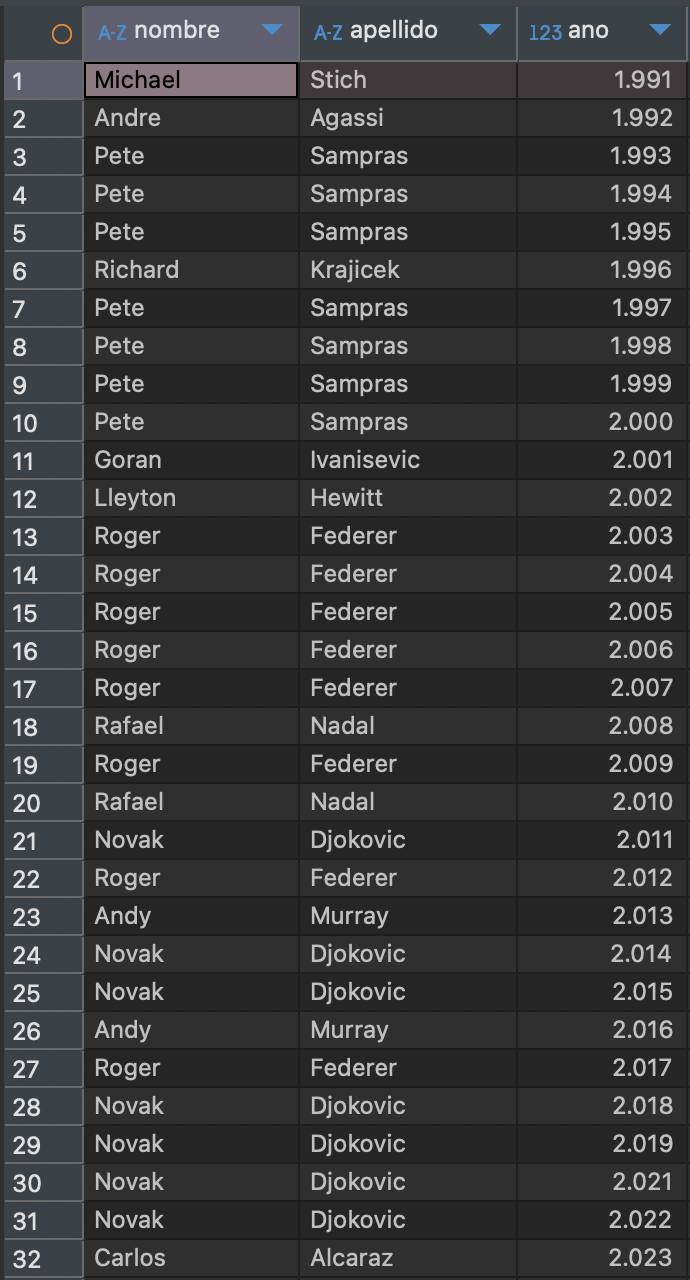
\includegraphics[height=0.4\textheight]{fotos/q1_com.png}
\caption{Datos agregados en SQL. Tipos compuestos, consulta 1.}
\label{fig:q1_com}
\end{figure}


\subsubsection{Muestra los años en los que Roger Federer ganó algún torneo de nivel Gran Slam (G) o Master 1000 (M). Para cada año, muestra el número de torneos y lista sus nombres (ordenados por la fecha de celebración). Ordena el resultado por el año}

Para reescribir esta consulta, usamos la única tabla de la que disponemos. Fijamos como condiciones de selección que el nombre del ganador sea Roger y el apellido Federer (campos a los que accedemos mediante \texttt{ganador}, que es un tipo compuesto), que el nivel del torneo sea G o M (accedemos a nivel mediante \texttt{(torneo).nivel}, ya que nivel es un campo del atributo \texttt{torneo}, de tipo \texttt{edicion\_torneo}) y que la ronda sea final (F). Esto nos devuelve una tupla para cada partido final de un Grand Slam o Master 1000 que Roger Federer ha ganado. Agrupamos esto por año, que lo obtenemos desde la fecha del torneo, a la cual accedemos a través del tipo \texttt{torneo} como \texttt{(torneo).fecha}, para obtener una única fila para cada año. Como proyección nos quedamos con el año del torneo (de los torneos concretamente), el número de torneos que hay en esa agrupación (los podemos contar por el número de \texttt{id} distintos que haya, accediendo a \texttt{(torneo).torneo.id}), y una concatenación del nombre de los torneos ganados ese año por Federer ordenada por fecha (el campo \texttt{nombre} lo encontramos, de nuevo, accediendo a \texttt{(torneo).torneo}). A continuación, mostramos la consulta y el resultado, que coincide con lo esperado, se puede ver en la figura \ref{fig:q2_com}.

\begin{minted}[frame=single, fontsize=\footnotesize]{sql}
select extract(year from (torneo).fecha) as ano, count(distinct (torneo).torneo.id) as numero_torneos, 
	string_agg((torneo).torneo.nombre, ', ' order by (torneo).fecha) as torneos
from partidos
where (torneo).nivel in ('G', 'M')
	and (ganador).nombre = 'Roger'
	and (ganador).apellido = 'Federer'
	and ronda = 'F'
group by ano
\end{minted}

\begin{figure}[H]
\centering
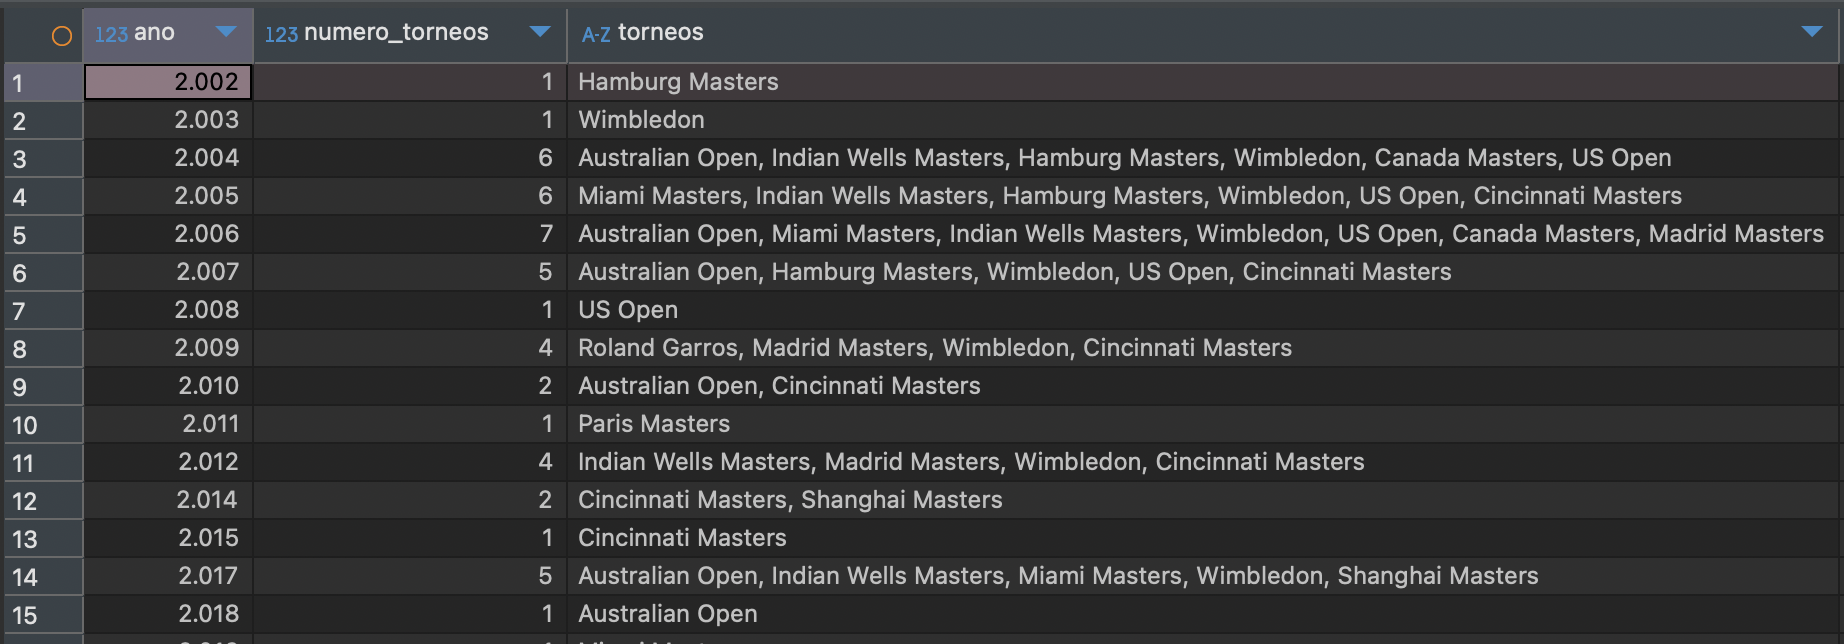
\includegraphics[width=0.8\textwidth]{fotos/q2_com.png}
\caption{Datos agregados en SQL. Tipos compuestos, consulta 2.}
\label{fig:q2_com}
\end{figure}





\subsubsection{Muestra los partidos de semifinales (ronda='SF') y final (ronda = 'F') del torneo de "Roland Garros" del 2018. Para cada partido muestra la ronda, el tipo de desenlace, el nombre y apellidos del ganador y el nombre y apellidos del perdedor y el resultado con el número de juegos del ganador y del perdedor en cada set, y opcionalmente en paréntesis el número de juegos del perdedor en el tie break}

En este caso, las condiciones de selección que deben ir en el \texttt{where} son la ronda (semifinal o final), el nombre del torneo (Roland Garros) y el año (2018). Para cada partido, queremos mostrar la ronda, el desenlace, el nombre y apellidos del ganador y del perdedor, y el resultado con el número de juegos del ganador y del perdedor en cada set. Para ello, debemos acceder a los campos de los tipos compuestos que hemos definido. Todo esto se obtiene de forma fácil y directa accediendo a las columnas necesarios, usando paréntesis en caso de que esa columna se un tipo compuesto, a excepción de la información de los sets. Veamos esto en concreto con un poco más de detalle. \\

Para obtener la información de los sets, debemos acceder a la columna \texttt{info\_sets}, que es un array con elementos de tipo compuesto. Para acceder a sus elementos, debemos hacer una subconsulta donde desagreguemos el array en el \texttt{from} con la función \texttt{unnest}. Tras desagregar el array, se trata como una consulta estándar y accedemos a los campos de los elementos del array como si fueran columnas de una tabla. En este caso, accedemos a los campos \texttt{juegos\_ganador}, \texttt{juegos\_perdedor} y \texttt{puntos\_tiebreak\_perdedor} de cada set. Para mostrar estos datos de forma más clara, concatenamos los resultados en un solo string con la función \texttt{string\_agg}, mostrando la puntuación del \textit{tiebreak} solo si existe. Además, esta concatenación se hace por orden ascendente según el número del set. Así, obtenemos una única tupla con los información de los sets de un partido. La consulta y el resultado, que coincide con lo esperado, se pueden ver en la figura \ref{fig:q3_com}.

\begin{minted}[frame=single, fontsize=\footnotesize]{sql}
select ronda, desenlace, 
	(ganador).nombre || ' ' || (ganador).apellido as ganador,
	(perdedor).nombre || ' ' || (perdedor).apellido as perdedor, 
	(select string_agg(iset.juegos_ganador || '-' || iset.juegos_perdedor ||
	case
		when iset.puntos_tiebreak_perdedor is not null then 
			'(' || iset.puntos_tiebreak_perdedor || ')'
		else ''
	end, ', ' order by iset.num_set) 
	from unnest(info_sets) as iset) as resultado
from partidos
where ronda in ('SF', 'F')
	and (torneo).torneo.nombre = 'Roland Garros'
	and extract(year from fecha) = '2018'
\end{minted}

\begin{figure}[H]
\centering
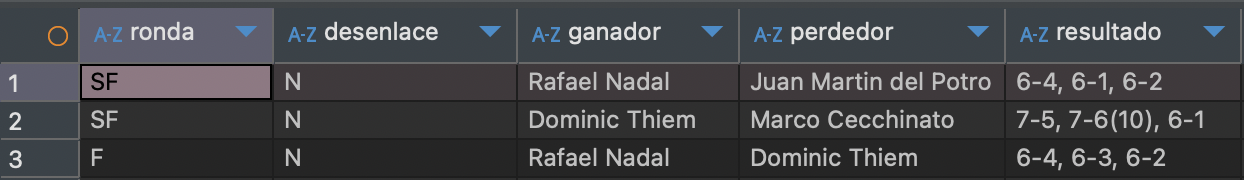
\includegraphics[width=0.7\textwidth]{fotos/q3_com.png}
\caption{Datos agregados en SQL. Tipos compuestos, consulta 3.}
\label{fig:q3_com}
\end{figure}




\subsubsection{Muestra la lista de jugadores españoles (ES) que ganaron algún torneo de nivel Gran Slam (G). Para cada jugador muestra los siguientes datos resumen de todos sus partidos: número de partidos jugados, porcentaje de victorias, porcentaje de aces, porcentaje de dobles faltas, porcentaje de servicios ganados, porcentaje de restos ganados, porcentaje de break points salvados (de los sufridos en contra), porcentaje de break points ganados (de los provocados a favor)}

Esta consulta, al igual que en el caso del modelo relacional, la dividiremos en dos partes, una para obtener los jugadores españoles que han ganado algún torneo de nivel Gran Slam y otra para obtener los datos resumen de todos sus partidos. Para la primera parte, usando la tabla \texttt{partidos} en el \texttt{from}, fijamos como condiciones de selección que el país del ganador sea España (accedemos a la columna de ganador y seleccionamos, del campo pais, el codigo iso 2), el nivel del torneo sea G y la ronda sea final. Esto nos devuelve una tupla por cada edicion del torneo ganado por un jugador español, por lo que en la proyección usaremos un \texttt{distinct} para quedarnos con una lista de jugadores únicos: queremos su \texttt{id} y su nombre completo, como concatenación de \texttt{nombre} y \texttt{apellido}. Todos estos campos son accesibles desde la columna \texttt{(ganador)}. El resultado será un tabla que llamaremos \texttt{jugadores\_espanoles\_ganadores}. \\

Para la segunda parte usaremos el producto cartesiano de \texttt{jugadores\_espanoles\_ganadores} y \texttt{partidos}. Como condiciones de \textit{join} usaremos los \texttt{id} de los jugadores, tanto del ganador como del perdedor. Estos son campos dentro de las columnas de tipo compuesto \texttt{p.ganador} y \texttt{p.perdedor}. Para obtener los datos resumen del partido en la proyección, usaremos un razonamiento análogo al que se usó en la consulta 3 del modelo relacional, por lo que no entrearemos a ese nivel de detalle. Sin embargo, comentamos los detalles técnicos que diferencian ambas consultas en este aspecto concreto: 
\begin{itemize}
\item Para verificar si el jugador español es el ganador o el perdedor, necesitamos recurrir a \texttt{id\_jugador}, de la tabla \texttt{jugadores\_espanoles\_ganadores} y el \texttt{id} del jugador, que encontramos como atributo del ganador o perdedor en la tabla \texttt{partidos}, que son columnas de tipo compuesto. 
\item Para acceder a las estadísticas, al ser columnas de tipo compuesto, debemos acceder usando también paréntesis, al igual que para los atributos del ganador o el perdedor, esto es \texttt{(p.ganador\_stats).} o \texttt{(p.perdedor\_stats).}
\end{itemize}

Teniendo en cuenta esto, la consulta se muestra a continuación y el resultado, que coincide con lo esperado, se pueden ver en la figura \ref{fig:q4_com}.

\begin{minted}[frame=single, fontsize=\footnotesize]{sql}
with jugadores_espanoles_ganadores as (
    select distinct (ganador).id as id_jugador, (ganador).nombre || ' ' || (ganador).apellido AS jugador
    from partidos
    where (ganador).pais.codigo_iso2 = 'ES'
        and ronda = 'F'
        and (torneo).nivel = 'G'
)

select
    jeg.jugador,
    count(p.num_partido) as partidos,
    round(100.0 * sum(case when jeg.id_jugador = (p.ganador).id then 1 else 0 end) / 
	count(p.num_partido), 1) as pcje_victorias,
    round(100.0 * sum(case when jeg.id_jugador = (p.ganador).id then (p.ganador_stats).num_aces 
	else (p.perdedor_stats).num_aces end) /
        nullif(sum(case when jeg.id_jugador = (p.ganador).id then (p.ganador_stats).num_ptos_servidos 
		else (p.perdedor_stats).num_ptos_servidos end), 0), 1) as pcje_aces,
    round(100.0 * sum(case when jeg.id_jugador = (p.ganador).id then (p.ganador_stats).num_dob_faltas 
	else (p.perdedor_stats).num_dob_faltas end) /
        nullif(sum(case when jeg.id_jugador = (p.ganador).id then (p.ganador_stats).num_ptos_servidos 
		else (p.perdedor_stats).num_ptos_servidos end), 0), 1) as pcje_dobles_faltas,
    round(100.0 * sum(case when jeg.id_jugador = (p.ganador).id 
	then (p.ganador_stats).num_primeros_servicios_ganados + 
	(p.ganador_stats).num_segundos_servicios_ganados
            else (p.perdedor_stats).num_primeros_servicios_ganados + 
			(p.perdedor_stats).num_segundos_servicios_ganados end) /
        nullif(sum(case when jeg.id_jugador = (p.ganador).id then (p.ganador_stats).num_ptos_servidos 
		else (p.perdedor_stats).num_ptos_servidos end), 0), 1) as pcje_servicios_ganados,
    round(100.0 * sum(case when jeg.id_jugador = (p.ganador).id
            then (p.perdedor_stats).num_ptos_servidos - (p.perdedor_stats).num_primeros_servicios_ganados - 
			(p.perdedor_stats).num_segundos_servicios_ganados
            else (p.ganador_stats).num_ptos_servidos - (p.ganador_stats).num_primeros_servicios_ganados - 
			(p.ganador_stats).num_segundos_servicios_ganados end) /
        nullif(sum(case when jeg.id_jugador = (p.ganador).id then (p.perdedor_stats).num_ptos_servidos 
		else (p.ganador_stats).num_ptos_servidos end), 0), 1) as pcje_restos_ganados,
    round(100.0 * sum(case when jeg.id_jugador = (p.ganador).id then (p.ganador_stats).num_break_salvados 
	else (p.perdedor_stats).num_break_salvados end) /
        nullif(sum(case when jeg.id_jugador = (p.ganador).id then (p.ganador_stats).num_break_afrontados 
		else (p.perdedor_stats).num_break_afrontados end), 0), 1) as pcje_breaks_salvados,
    round(100.0 * sum(case when jeg.id_jugador = (p.ganador).id then (p.perdedor_stats).num_break_afrontados 
	- (p.perdedor_stats).num_break_salvados
            else (p.ganador_stats).num_break_afrontados - (p.ganador_stats).num_break_salvados end) /
        nullif(sum(case when jeg.id_jugador = (p.ganador).id then (p.perdedor_stats).num_break_afrontados 
		else (p.ganador_stats).num_break_afrontados end), 0), 1) as pcje_breaks_ganados
from jugadores_espanoles_ganadores jeg, partidos p
where jeg.id_jugador = (p.ganador).id
    or jeg.id_jugador = (p.perdedor).id
group by jeg.jugador
\end{minted}

\begin{figure}[H]
\centering
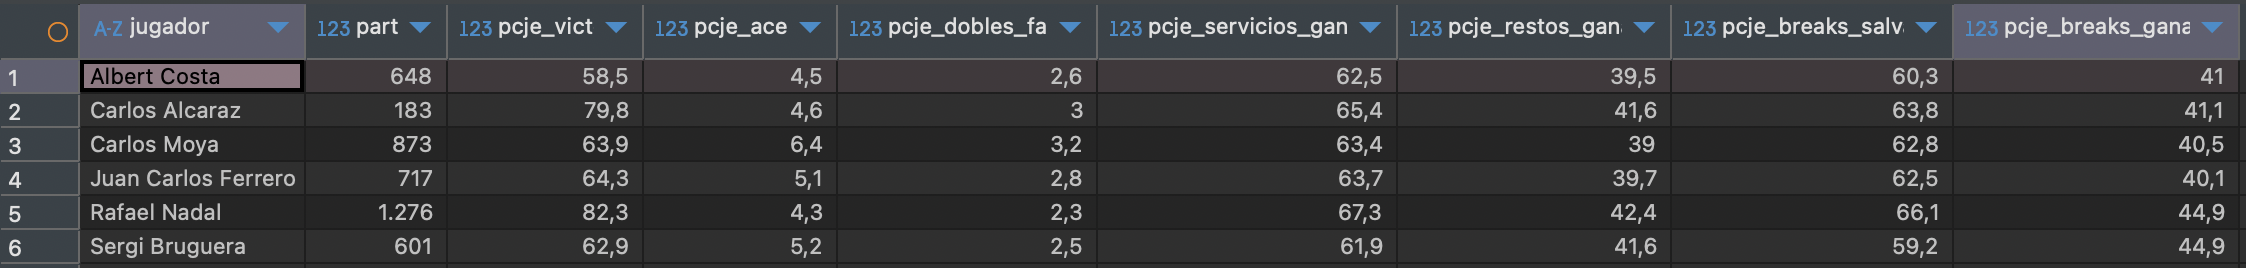
\includegraphics[width=\textwidth]{fotos/q4_com.png}
\caption{Datos agregados en SQL. Tipos compuestos, consulta 4.}
\label{fig:q4_com}
\end{figure}





\subsubsection{Lista los jugadores que fueron derrotados (en algún partido del 2018) por el rival de Rafael Nadal de la primera ronda (R128) de Roland Garros de 2018}

Esta consulta la dividiremos en dos subconsultas, una para obtener el rival de Rafael Nadal en la primera ronda de Roland Garros de 2018 y otra para obtener los jugadores que fueron derrotados por ese rival. Para la primera parte, que solo requiere la tabla \texttt{partidos}, fijamos como condiciones de selección que la ronda sea R128, el nombre del torneo sea Roland Garros y el año sea 2018. Además, el nombre del ganador o perdedor debe ser Rafael, y su apellido Nadal. No explicamos cómo acceder a estos campos porque ya se hizo con anterioridad. Esto devuelve una única fila con el rival de Nadal en este partido concreto, por lo que nos quedamos únicamente con la proyección de su nombre completo (concatenación de \texttt{nombre} y \texttt{apellido}). La tabla resultante la llamaremos \texttt{rival\_nadal}. \\

Para la segunda parte, usaremos el producto cartesiano de \texttt{rival\_nadal} y \texttt{partidos}. Como condiciones de \textit{join} usaremos que el nombre y apellido del rival de Nadal coincida con el nombre y apellidos del ganador de ese partido, que es una columna de tipo compuesto (\texttt{ganador}) a la cual accedemos como en las consultas anteriores. Además, si seleccionamos los partidos disputados en 2018 a través de la fecha, obtenemos un conjunto de tuplas con los partidos ganados por el rival de Nadal en 2018. En la proyección, nos quedamos simplemente con una concatenación del nombre y apellido del perdedor y su país, al que accedemos a través de \texttt{(perdedor).pais.codigo\_iso2}. No haría falta, pero ordenamos el resultado por el nombre del jugador. La consulta y el resultado, que coincide con el esperado, se pueden ver en la figura \ref{fig:q5_com}.

\begin{minted}[frame=single, fontsize=\footnotesize]{sql}
with rival_nadal as (
	select case when (ganador).nombre = 'Rafael' then (perdedor).nombre || ' ' || (perdedor).apellido 
		else (ganador).nombre || ' ' || (ganador).apellido end as jugador
	from partidos 
	where (((ganador).nombre = 'Rafael' and (ganador).apellido = 'Nadal') or 
		((perdedor).nombre = 'Rafael' and(perdedor).apellido = 'Nadal'))
		and ronda = 'R128'
		and (torneo).torneo.nombre = 'Roland Garros'
		and extract(year from fecha) = '2018'
)

select (p.perdedor).nombre || ' ' || (p.perdedor).apellido as jugador, (p.perdedor).pais.codigo_iso2 as pais
from partidos p, rival_nadal rn
where (p.ganador).nombre || ' ' || (p.ganador).apellido = rn.jugador
	and extract(year from p.fecha) = '2018'
order by jugador
\end{minted}


\begin{figure}[H]
\centering
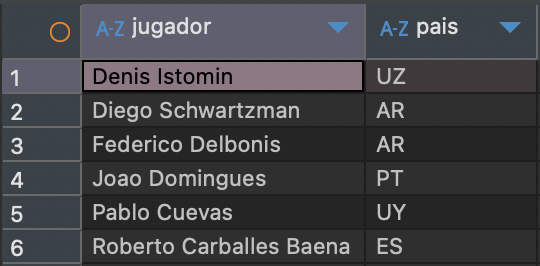
\includegraphics[width=0.35\textwidth]{fotos/q5_com.png}
\caption{Datos agregados en SQL. Tipos compuestos, consulta 5.}
\label{fig:q5_com}
\end{figure}
